%==============================================================================
% tento soubor pouzijte jako zaklad
% this file should be used as a base for the thesis
% Autoři / Authors: 2008 Michal Bidlo, 2019 Jaroslav Dytrych
% Kontakt pro dotazy a připomínky: sablona@fit.vutbr.cz
% Contact for questions and comments: sablona@fit.vutbr.cz
%==============================================================================
% kodovani: UTF-8 (zmena prikazem iconv, recode nebo cstocs)
% encoding: UTF-8 (you can change it by command iconv, recode or cstocs)
%------------------------------------------------------------------------------
% zpracování / processing: make, make pdf, make clean
%==============================================================================
% Soubory, které je nutné upravit nebo smazat: / Files which have to be edited or deleted:
%   xberna18-20-literatura-bibliography.bib - literatura / bibliography
%   xberna18-01-kapitoly-chapters.tex - obsah práce / the thesis content
%   xberna18-01-kapitoly-chapters-en.tex - obsah práce v angličtině / the thesis content in English
%   xberna18-30-prilohy-appendices.tex - přílohy / appendices
%   xberna18-30-prilohy-appendices-en.tex - přílohy v angličtině / appendices in English
%==============================================================================
\documentclass[zadani]{fitthesis} % odevzdani do wisu a/nebo tisk s barevnými odkazy - odkazy jsou barevné
% \documentclass[zadani,cprint]{fitthesis} % pro barevný tisk - odkazy jsou černé, znak VUT barevný
% \documentclass[zadani,cprint,twoside]{fitthesis} % pro barevný tisk - odkazy jsou černé, znak VUT barevný

%\documentclass[]{fitthesis} % bez zadání - pro začátek práce, aby nebyl problém s překladem
%\documentclass[english]{fitthesis} % without assignment - for the work start to avoid compilation problem
%\documentclass[english,zadani]{fitthesis} % for submission to the IS FIT and/or print with color links - links are color
%\documentclass[zadani,print]{fitthesis} % pro černobílý tisk - odkazy jsou černé
%\documentclass[english,zadani,print]{fitthesis} % for the black and white print - links are black
%\documentclass[english,zadani,cprint]{fitthesis} % for the print - links are black, logo is color
% * Je-li práce psaná v anglickém jazyce, je zapotřebí u třídy použít 
%   parametr english následovně:
%   If thesis is written in English, it is necessary to use 
%   parameter english as follows:
%      \documentclass[english]{fitthesis}
% * Je-li práce psaná ve slovenském jazyce, je zapotřebí u třídy použít 
%   parametr slovak následovně:
%   If the work is written in the Slovak language, it is necessary 
%   to use parameter slovak as follows:
%      \documentclass[slovak]{fitthesis}
% * Je-li práce psaná v anglickém jazyce se slovenským abstraktem apod., 
%   je zapotřebí u třídy použít parametry english a enslovak následovně:
%   If the work is written in English with the Slovak abstract, etc., 
%   it is necessary to use parameters english and enslovak as follows:
%      \documentclass[english,enslovak]{fitthesis}

% Základní balíčky jsou dole v souboru šablony fitthesis.cls
% Basic packages are at the bottom of template file fitthesis.cls
% zde můžeme vložit vlastní balíčky / you can place own packages here

% Kompilace po částech (rychlejší, ale v náhledu nemusí být vše aktuální)
% Compilation piecewise (faster, but not all parts in preview will be up-to-date)
% \usepackage{subfiles}

% Nastavení cesty k obrázkům
% Setting of a path to the pictures
%\graphicspath{{obrazky-figures/}{./obrazky-figures/}}
%\graphicspath{{obrazky-figures/}{../obrazky-figures/}}

%---rm---------------
\renewcommand{\rmdefault}{lmr}%zavede Latin Modern Roman jako rm / set Latin Modern Roman as rm
%---sf---------------
\renewcommand{\sfdefault}{qhv}%zavede TeX Gyre Heros jako sf
%---tt------------
\renewcommand{\ttdefault}{lmtt}% zavede Latin Modern tt jako tt

% vypne funkci šablony, která automaticky nahrazuje uvozovky,
% aby nebyly prováděny nevhodné náhrady v popisech API apod.
% disables function of the template which replaces quotation marks
% to avoid unnecessary replacements in the API descriptions etc.
\csdoublequotesoff

% =======================================================================
% balíček "hyperref" vytváří klikací odkazy v pdf, pokud tedy použijeme pdflatex
% problém je, že balíček hyperref musí být uveden jako poslední, takže nemůže
% být v šabloně
% "hyperref" package create clickable links in pdf if you are using pdflatex.
% Problem is that this package have to be introduced as the last one so it 
% can not be placed in the template file.
\ifWis
\ifx\pdfoutput\undefined % nejedeme pod pdflatexem / we are not using pdflatex
\else
  \usepackage{color}
  \usepackage[unicode,colorlinks,hyperindex,plainpages=false,pdftex]{hyperref}
  \definecolor{hrcolor-ref}{RGB}{223,52,30}
  \definecolor{hrcolor-cite}{HTML}{2F8F00}
  \definecolor{hrcolor-urls}{HTML}{092EAB}
  \hypersetup{
	linkcolor=hrcolor-ref,
	citecolor=hrcolor-cite,
	filecolor=magenta,
	urlcolor=hrcolor-urls
  }
  \def\pdfBorderAttrs{/Border [0 0 0] }  % bez okrajů kolem odkazů / without margins around links
  \pdfcompresslevel=9
\fi
\else % pro tisk budou odkazy, na které se dá klikat, černé / for the print clickable links will be black
\ifx\pdfoutput\undefined % nejedeme pod pdflatexem / we are not using pdflatex
\else
  \usepackage{color}
  \usepackage[unicode,colorlinks,hyperindex,plainpages=false,pdftex,urlcolor=black,linkcolor=black,citecolor=black]{hyperref}
  \definecolor{links}{rgb}{0,0,0}
  \definecolor{anchors}{rgb}{0,0,0}
  \def\AnchorColor{anchors}
  \def\LinkColor{links}
  \def\pdfBorderAttrs{/Border [0 0 0] } % bez okrajů kolem odkazů / without margins around links
  \pdfcompresslevel=9
\fi
\fi
% Řešení problému, kdy klikací odkazy na obrázky vedou za obrázek
% This solves the problems with links which leads after the picture
\usepackage[all]{hypcap}

% Informace o práci/projektu / Information about the thesis
%---------------------------------------------------------------------------
\projectinfo{
  %Prace / Thesis
  project={BP},            %typ práce BP/SP/DP/DR  / thesis type (SP = term project)
  year={2021},             % rok odevzdání / year of submission
  date=\today,             % datum odevzdání / submission date
  %Nazev prace / thesis title
  title.cs={Aplikace pro řízený přístup ke vzdáleným dokumentům pro GNU/Linux},  % název práce v češtině či slovenštině (dle zadání) / thesis title in czech language (according to assignment)
  title.en={Application for Controlled Access to Remote Documents for GNU/Linux}, % název práce v angličtině / thesis title in english
  %title.length={14.5cm}, % nastavení délky bloku s titulkem pro úpravu zalomení řádku (lze definovat zde nebo níže) / setting the length of a block with a thesis title for adjusting a line break (can be defined here or below)
  %sectitle.length={14.5cm}, % nastavení délky bloku s druhým titulkem pro úpravu zalomení řádku (lze definovat zde nebo níže) / setting the length of a block with a second thesis title for adjusting a line break (can be defined here or below)
  %Autor / Author
  author.name={Jan},   % jméno autora / author name
  author.surname={Bernard},   % příjmení autora / author surname 
  %author.title.p={Bc.}, % titul před jménem (nepovinné) / title before the name (optional)
  %author.title.a={Ph.D.}, % titul za jménem (nepovinné) / title after the name (optional)
  %Ustav / Department
  department={UIFS}, % doplňte příslušnou zkratku dle ústavu na zadání: UPSY/UIFS/UITS/UPGM / fill in appropriate abbreviation of the department according to assignment: UPSY/UIFS/UITS/UPGM
  % Školitel / supervisor
  supervisor.name={Marek},   % jméno školitele / supervisor name 
  supervisor.surname={Rychlý},   % příjmení školitele / supervisor surname
  supervisor.title.p={RNDr.},   %titul před jménem (nepovinné) / title before the name (optional)
  supervisor.title.a={Ph.D.},    %titul za jménem (nepovinné) / title after the name (optional)
  % Klíčová slova / keywords
  keywords.cs={Validované datové uložiště, VDU, Linux, souborový systém, HTTP, FUSE, C++, synchronizace, soubor, dokument, oprávnění }, % klíčová slova v českém či slovenském jazyce / keywords in czech or slovak language
  keywords.en={Validated data storage, VDS, Linux, filesystem, HTTP, FUSE, C++, synchronization, file, document, permission }, % klíčová slova v anglickém jazyce / keywords in english
  %keywords.en={Here, individual keywords separated by commas will be written in English.},
  % Abstrakt / Abstract
  abstract.cs={
    Práce se zaměřuje na synchronizaci a životní cyklus souborů stažených do uživatelského počítače ze vzdáleného validovaného datového uložiště.
    Z analýzy trhu vyplynulo, že na trhu je velký výběr aplikací, ale rozdíly mezi nimi jsou relativně velké. Na základě požadavků a stanovené komunikace s validovaným datovým
    uložištěm byla navržena a implementována aplikace pro systém \mbox{GNU/Linux}. Testování aplikace probíhalo na dvou vybraných Linuxových distribucích
    s mock serverem zastupující vzdálené uložiště.
  }, % abstrakt v českém či slovenském jazyce / abstract in czech or slovak language
  abstract.en={
    The aim of this thesis is synchronization and life cycle of files downloaded to user's computer from validated data storage. Based on market analysis
    there is large selection of applications in market but there are relatively large differences along them. Application was designed and implemented for GNU/Linux
    according to requirements and given validated data storage communication. The application was tested on two selected Linux distributions with Mock Server
    represententing remote storage.
  }, % abstrakt v anglickém jazyce / abstract in english
  %abstract.en={An abstract of the work in English will be written in this paragraph.},
  % Prohlášení (u anglicky psané práce anglicky, u slovensky psané práce slovensky) / Declaration (for thesis in english should be in english)
  declaration={Prohlašuji, že jsem tuto bakalářskou práci vypracoval samostatně pod vedením pana RNDr. Marka Rychlého, Ph.D. a uvedl jsem všechny literární prameny, publikace a další zdroje, ze kterých jsem čerpal.},
  %declaration={I hereby declare that this Bachelor's thesis was prepared as an original work by the author under the supervision of Mr. X
% The supplementary information was provided by Mr. Y
% I have listed all the literary sources, publications and other sources, which were used during the preparation of this thesis.},
  % Poděkování (nepovinné, nejlépe v jazyce práce) / Acknowledgement (optional, ideally in the language of the thesis)
  acknowledgment={
    Rád bych poděkoval vedoucímu práce, doktorovi Markovi Rychlému, za vynikající vedení práce a jeho podnětné poznatky a rady. Také bych rád poděkoval všem svým kolegům,
    se kterými jsem procházel celé bakalářské studium. A v neposlední řadě děkuji všem svým přátelům a rodině za podporu a pochopení.
  },
  %acknowledgment={Here it is possible to express thanks to the supervisor and to the people which provided professional help
%(external submitter, consultant, etc.).},
  % Rozšířený abstrakt (cca 3 normostrany) - lze definovat zde nebo níže / Extended abstract (approximately 3 standard pages) - can be defined here or below
  %extendedabstract={Do tohoto odstavce bude zapsán rozšířený výtah (abstrakt) práce v českém (slovenském) jazyce.},
  %faculty={FIT}, % FIT/FEKT/FSI/FA/FCH/FP/FAST/FAVU/USI/DEF
  faculty.cs={Fakulta informačních technologií}, % Fakulta v češtině - pro využití této položky výše zvolte fakultu DEF / Faculty in Czech - for use of this entry select DEF above
  faculty.en={Faculty of Information Technology}, % Fakulta v angličtině - pro využití této položky výše zvolte fakultu DEF / Faculty in English - for use of this entry select DEF above
  department.cs={Ústav matematiky}, % Ústav v češtině - pro využití této položky výše zvolte ústav DEF nebo jej zakomentujte / Department in Czech - for use of this entry select DEF above or comment it out
  department.en={Institute of Mathematics} % Ústav v angličtině - pro využití této položky výše zvolte ústav DEF nebo jej zakomentujte / Department in English - for use of this entry select DEF above or comment it out
}

% Rozšířený abstrakt (cca 3 normostrany) - lze definovat zde nebo výše / Extended abstract (approximately 3 standard pages) - can be defined here or above
%\extendedabstract{Do tohoto odstavce bude zapsán výtah (abstrakt) práce v českém (slovenském) jazyce.}

% nastavení délky bloku s titulkem pro úpravu zalomení řádku - lze definovat zde nebo výše / setting the length of a block with a thesis title for adjusting a line break - can be defined here or above
%\titlelength{14.5cm}
% nastavení délky bloku s druhým titulkem pro úpravu zalomení řádku - lze definovat zde nebo výše / setting the length of a block with a second thesis title for adjusting a line break - can be defined here or above
%\sectitlelength{14.5cm}

% řeší první/poslední řádek odstavce na předchozí/následující stránce
% solves first/last row of the paragraph on the previous/next page
\clubpenalty=10000
\widowpenalty=10000

% checklist
\newlist{checklist}{itemize}{1}
\setlist[checklist]{label=$\square$}

\begin{document}
  % Vysazeni titulnich stran / Typesetting of the title pages
  % ----------------------------------------------
  \maketitle
  % Obsah
  % ----------------------------------------------
  \setlength{\parskip}{0pt}

  {\hypersetup{hidelinks}\tableofcontents}
  
  % Seznam obrazku a tabulek (pokud prace obsahuje velke mnozstvi obrazku, tak se to hodi)
  % List of figures and list of tables (if the thesis contains a lot of pictures, it is good)
  \ifczech
    \renewcommand\listfigurename{Seznam obrázků}
  \fi
  \ifslovak
    \renewcommand\listfigurename{Zoznam obrázkov}
  \fi
  % {\hypersetup{hidelinks}\listoffigures}
  
  \ifczech
    \renewcommand\listtablename{Seznam tabulek}
  \fi
  \ifslovak
    \renewcommand\listtablename{Zoznam tabuliek}
  \fi
  % {\hypersetup{hidelinks}\listoftables}

  \ifODSAZ
    \setlength{\parskip}{0.5\bigskipamount}
  \else
    \setlength{\parskip}{0pt}
  \fi

  % vynechani stranky v oboustrannem rezimu
  % Skip the page in the two-sided mode
  \iftwoside
    \cleardoublepage
  \fi

  % Text prace / Thesis text
  % ----------------------------------------------
  \ifenglish
    \input{xberna18-01-kapitoly-chapters-en}
  \else
    \chapter{Úvod}

V době vysokorychlostního a stabilního internetu je využívání vzdálených uložišť běžnou záležitostí. Pro většinu uživatelů je to nástroj
pro jednoduchou synchronizaci dat napříč několika zařízeními od mobilního telefonu po stolní počítač. Pokud vezmeme v úvahu pouze velká datová centra,
jedná se pravděpodobně o nejlevnější a nejspolehlivější způsob uchování dat, protože tyto centra mají velkou kapacitu úložného prostoru a také zálohy na
softwarové i hardwarové úrovni. Pod pojmem vzdálené uložiště si nemusíme představit jen velká datová centra se stovkami serverů, může se jednat o relativně malé uložiště
ve firmě nebo dokonce o osobní/domácí řešení. Pro využívání osobních/firemních uložišť se lidé uchylují v případech, je-li třeba uložit osobní nebo
určitým způsobem citlivá data, která by nemohla být poskytnuta třetí straně. Nabízená řešení také nemusí poskytovat potřebnou funkcionalitu nebo jejich finanční model
nesplňuje zákazníkova kritéria.

V průběhu let byly vyvinuty protokoly řešící sdílení souborů jako FTP, NFS a mnohé další. Sdílení souborů je komplexní záležitostí a obsahuje
velké množství parametrů. Každý protokol se zaměřuje jen na určité parametry jako zabezpečení a spolehlivost přenosu, oprávnění pro jednotlivé
uživatele a soubory, synchronizace modifikovaných souborů apod. nebo pojme daný parametr odlišným způsobem. V dnešní době je většina komerčně využívaných
aplikací vystavěna na proprietárních protokolech, nebo na protokolech umožňující obecnější použití. Jedním z nejpoužívanějších aplikačních protokolů
bude Hypertext Transfer Protokol neboli HTTP.

Cílem této práce je prozkoumat aktuální nabídku a možnosti na poli vzdálených uložišť a navrhnout aplikaci pro řízený přístup ke vzdáleným dokumentům pro
platformu \mbox{GNU/Linux}. Aplikace bude zaměřena na řízený životní cyklus souborů s vynucenými oprávněními pro jednotlivé soubory daná vzdáleným uložištěm.
Komunikace skrze HTTP protokol byla definovaná externím zadavatelem. Zdrojové kódy jsou dostupné na veřejném Github repozitáři.
\footnote{\url{https://github.com/PlayerBerny12/VUT-IBT-Code}}

% ---------------------------------------------------------------------------------------------------------------------------------------
\chapter{Motivace a existující řešení}

Popularita a využití vzdálených uložišť roste, protože lidé využívají více zařízení a potřebují mezi nimi jednoduchou synchronizaci nebo na jednom souboru
potřebuje spolupracovat více lidí. Dalším podnětem využívání vzdálených uložišť je větší množství dat a potřeba tyto data efektivně sdílet a bezpečně uložit.
Postupně se digitalizují další systémy například ve státní správě nebo dalších podnikatelských sektorech. 

Na trhu je velké množství služeb zaměřujících se na různé klientské potřeby. Diverzita nabídky je až překvapivě velká. Většina se zaměřuje na ukládání a sdílení
dat ve svém ekosystému, které jsou určené pro široké použití. Pokud jsou požadavky specifické, tak možnost vlastní konfigurace není možná. Pro částečnou úpravu 
nebo automatizaci procesů lze využít poskytované API, ve většině případu se jedná o variantu REST API. Poslední možností je vystavění obdobné služby z několika
existujících aplikací nebo vytvoření nové.\\

\noindent V kontextu této práce jsou požadavky následující: 

\begin{itemize}
    \item Dodržování oprávnění i na klientském systému
    \begin{itemize}
        \item read-only
        \item write-only
        \item read + write
    \end{itemize}
    \item Životní cyklus souboru (stažení)
    \begin{itemize}
        \item stažení
        \item případná modifikace
        \item smazání souboru po vypršení platnosti
    \end{itemize}
    \item Autentifikace
    \begin{itemize}
        \item uživatelské jméno a klientský certifikát
        \item uživatelské jméno a heslo
    \end{itemize}
\end{itemize}

\section{Současná řešení}

Pro bližší analýzu byl vybrán vzorek služeb a programů obsahující velké ekosystémy služeb po open source aplikace. Zkoumáno bylo několik parametrů,
jako poskytovaná funkcionalita pro jednotlivce a firmy, cena, integrace s ostatními systémy a aplikacemi apod. Obecně nelze jednoznačně určit nejlepší uložiště, 
ale je možné poukázat na rozdílné vlastnosti a vyzdvihnout kladné. Koncový uživatel se následně může rozhodnout dle svých potřeb.

\section{Google Drive}

Pro synchronizaci obsahu z Google Drive na osobní počítač se využívá aplikace pojmenovaná Google File Stream. Je možné ji provozovat pouze na systémech
Windows a Mac OS. \cite{GoogleFileStream} Pro Linuxové distribuce lze využít například neoficiální open source aplikaci 
Google Drive OCamlFUSE\footnote{\url{https://github.com/astrada/google-drive-ocamlfuse}} využívající technologii
FUSE, která bude popsána v následující kapitole \ref{sec:fuse}. Google Disk poskytuje plně funkční webové rozhraní,
ve kterém je možné dokumenty přímo upravovat bez nutnosti stahování. Problém nenastal ani v případě konkurenčních Microsoft Office dokumentů. 

Google Workspace (dříve Google Suite) je možné pořídit v několika balíčcích. Například balíček Bussiness Standard nabízí 2 TB uložiště za 10,40 EUR měsíčně.
Balíček obsahuje další služby jako firemní email a schůzky až o 150 účastnících na Google Meet. \cite{GoogleWorkspace}

Každý uživatel má vlastní disk s omezenou kapacitou podle balíčku. Na disku lze vytvářet standartní složkovou hierarchii a je možné sdílet jednotlivé soubory nebo
obsah složek s ostatními Google uživateli. Verze Enterprise umožňuje vytváření dalších disků, na které je možné přiřadit seznam uživatelů. Každý uživatel
má nastavenou jednu z 6 rolí, které vymezují jeho možnosti. K dispozici je API, která pokrývá veškeré možnosti webového rozhraní jako vytvoření souboru,
sdílení atd. \cite{GoogleAPIReference}

\section{Dropbox}

Dropbox má oficiální balíčky své aplikace pro Ubuntu a Fedoru, případně je možné si aplikaci zkompilovat ze zdrojových souborů. Podpora Windows a Mac OS je samozřejmostí.
Z práce „Personal Cloud Storage Benchmarks and Comparison“ lze vyčíst, že Dropbox se zaměřuje na efektivitu přenosu a minimální zatížení sítě.
Využívá menší množství TCP spojení oproti jeho konkurentům a také stejně jako Google Drive komprimuje data před odesláním. \cite{CloudStorageComparison}
Toto řešení nemusí dosahovat nejvyšší výkonosti, ale nezatěžuje tolik infrastrukturu. 

Webové rozhraní je více orientováno na správu souborů a jejich historii. Nabízí jednoduché obnovení smazaných souborů nebo návrat k předchozí verzi.
Nenabízí tolik možností jako Google Drive, ale upravovat dokumenty ve webovém prohlížeči lze také. Na výběr je mezi Microsoft Office Online nebo Google Worksapce.
Sdílení souborů a složek je možné i s uživateli, kteří nemají Dropbox účet.

Balíček Plus za 9,99 EUR měsíčně dává uživateli přístup ke 2 TB uložišti. Firemní balíčky obsahují rozšíření pro lepší správu uživatelů, vytváření skupin
a admin panel/konzole. Dropbox má také API nabízející dostatečnou funkcionalitu pro případnou integraci s jinými systémy apod. \cite{Dropbox}

\section{pCloud}

Poskytovatel pCloud podporuje nejpoužívanější platformy, a to včetně mobilních. Za 9,99 EUR měsíčně dostane uživatel 2 TB uložiště. Jako jediný z poskytovatelů
v analýze nabízí balíček s jednorázovou platbou za cenu 350 EUR. Jedná se o identický balíček, pouze forma platby se liší. Všechna data jsou přenášena přes
šifrovaný kanál a všechny kopie souborů na pěti různých serverech jsou šifrovaná 256bitovým AES klíčem. \cite{pCloud}

Webové rozhraní je jednoduché, avšak oproti konkurentům má méně funkcí. Lze zobrazit náhled dokumentů, ale upravovat je nelze. Každý soubor má tzv. revize 
a je možné obnovit obsah souboru na vybranou revizi. Revize jsou uchovány po dobu jednoho roku. Soubory je možné sdílet i s uživateli, kteří nemají účet u pCloudu. 

Pro firemní zákazníky je nabízený rozšířený management uživatelů a monitoring s logy aktivity jednotlivých uživatelů.

\section{Syncthing}

Open source aplikace Syncthing synchronizuje soubory peer-to-peer. Nejedná se o čistou peer-to-peer architekturu, protože jeden z uzlů může být
nastaven jako server a veškerá data budou synchronizována vůči tomuto uzlu. Syncthing je možné provozovat na většině dnešních systémů jako Windows, Linux, BSD a Mac OS. \cite{Syncthing}

Aplikace poskytuje webové rozhraní, které je určené pouze pro nastavení parametrů jako discovery protokolu pro objevování ostatních uzlů, jaké složky mají být synchronizovány,
nebo kolik verzí jednotlivých souborů má být uchováváno a mnoho dalšího. Velká přizpůsobivost umožňuje upravit fungování aplikace vlastním potřebám, na druhou
stranu bude náročné udržovat systém s větším množstvím uživatelů vystavěný na této aplikaci. Jedná se tedy spíše o domácí řešení.

\section{Shrnutí}

Trendy na poli vzdálených uložišť určují velké firmy jako Google nebo Micorsoft. Důkazem tohoto jevu je například integrace aplikací obou těchto firem do webového
rozhraní Dropboxu. Aplikace One Drive od Microsoftu nebyla blíže analyzovaná, protože se jedná o službu pouze pro platformu Windows. 

Všechny služby mají webové rozhraní, ke kterému je aplikace synchronizující obsah uložiště občas brána jako doplněk. Sdílení nebo obnova předchozí verze souboru
je vždy možná ve webové aplikaci, ale ne vždy jsou tyto akce dostupné i na desktopové verzi.

Aplikace na jejímž základě je vytvořená tato práce nebude synchronizovat celé uložiště, ale bude pracovat jen s jednotlivými soubory. Uživateli na vyžádání stáhne 
právě jeden soubor, se kterým bude chtít uživatel v danou dobu pracovat (zobrazit nebo upravit obsah). Synchronizace celého uložiště nebo obsahu jedné složky nebude možná.
Jedná se spíše o náhradu možnosti zobrazovat a upravovat soubor přímo ve webovém prohlížeči jako to umožňuje například Google Drive.

% ---------------------------------------------------------------------------------------------------------------------------------------
\chapter{Návrh řešení a použité technologie}

Prvním krokem navrhovací fáze bylo seznámení se zadáním a požadavky. Externí zadavatel dodal podrobnou dokumentaci REST API pro validované datové uložiště, která
byla stěžejním dokumentem při návrhu. Jednalo se o formální textový popis, který nebyl v žádném standardizovaném formát. API obsahuje funkce pro ověření spojení,
autentifikaci a práci se soubory. VDU nebylo při vzniku této práce k dispozici, proto byl pro potřeby vývoje vytvořen Mock Server na základě přepisu poskytnuté
dokumentace do standardizovaného formátu OpenAPI.

Pro vynucení práv jednotlivých souborů je standartní souborový systém nevyhovující, protože po stažení souboru do počítače uživatele ztrácí VDU kontrolu nad tímto
souborem. Po konzultaci s vedoucím práce, doktorem Markem Rychlým, byla zvolena technologie FUSE neboli Filesystem in userspace. FUSE umožňuje vytvořit virtuální
souborový systém a implementovat jednotlivé operace jako čtení, zápis atd. Tím je možné dosáhnout dostatečnou kontrolu nad oprávněními a obecně životním cyklem souboru
v uživatelově počítači. Znalý uživatel by byl schopen tento systém obejít a přistoupit k souborům z hostovaného souborového systému. K takové operaci jsou však potřeba 
oprávnění superuživatele \texttt{root}.

\section{Případy užití}

Na základě požadavků bylo možné přímo vytvořit diagram případu užití. Pouze jedna věc nebyla konkrétně specifikovaná. Webová aplikace musí předat té desktopové 
přístupový token, pomocí kterého lze volat potřebné API metody VDU. V úvahu přišlo stažení „fake“ souboru obsahující pouze přístupový token. Druhou možností bylo
přesměrování na speciální URL z VDU. Prohlížeč by na základě přesměrování rozpoznal, že má otevřít určenou aplikaci a předat ji token jako jeden z parametrů
volání. Varianta se speciální URL působí na uživatele mnohem ucelenějším dojmem a nevytváří na souborovém systém dále nepotřebné soubory.

Diagram případů užití zachycuje celý systém jako celek a zobrazuje jednotlivé funkce a jejich návaznosti, které je třeba dále analyzovat a specifikovat v dalších
fázích návrhu. V diagramu \ref{fig:use_case} vystupují tři aktéři a to uživatel, FUSE agent/démon a VDU. Implementace VDU není obsahem této práce, proto je oddělena červenou
přerušovanou čarou. Autentifikace, na které závisí veškerá komunikace s VDU, není zanesená do diagramu. Díky této operaci byla zvýšena přehlednost diagramu.

\begin{figure*}[h]
    \centering    
    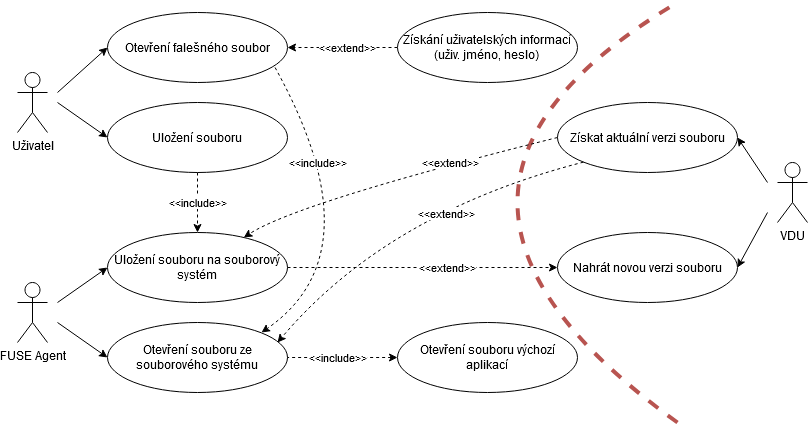
\includegraphics[width=1\linewidth]{other-fig/use_case_diagram.png}
    \caption{Diagram případu užití.}
    \label{fig:use_case}
\end{figure*}


Všechny akce jsou spuštěny uživatelem a většina z nich vyvolá reakci FUSE démona. Jedná se například o uložení, otevření nebo přejmenování souboru ve virtuálním souborovém
systému. Speciální případ nastává při otevření URL s vlastním protokolem, který má zavolat aplikaci, jež je k danému protokolu v systému přiřazena. Příkladem takového
protokolu může být \texttt{mailto}, využívaný často u webových stránek. Přesměrování na adresu s tímto protokolem otevře správce elektronické pošty. 

K námi definovanému protokolu pojmenovaném \texttt{vdu} je třeba mít v systému přiřazenou aplikaci, která pomocí přístupového tokenu uloženého v URL 
(\texttt{\mbox{vdu://<přístupový token>}}) stáhne žádaný soubor z VDU na virtuální souborový systém. Na základě této znalosti byly uskutečněny rozhodnutí při návrhu architektury.
 
\section{Definice REST API}

API obsahuje sedm metod pro ověření dostupnosti, autentifikaci a práci se soubory. Každá funkce má sadu možných návratových hodnot, která je podmnožinou návratových hodnot
definovaných protokolem HTTP. Podle tohoto kódu lze rozpoznat, zda bylo dané volaní úspěšné, případně jaká chyba při volání nastala. Kódy z rozsahu 200 až 299 označují
úspěšná volání a kódy 400 až 599 indikují chybu na straně klienta nebo serveru.

Standardizace definice REST API byla vytvořena v OpenAPI standardu, pro který je dostupných mnoho nástrojů. Jedním z nich je open source nástroj Swagger, pomocí kterého
můžete generovat HTML dokumentaci. Vygenerované rozhraní umožňuje i jednoduchou formu testování API. Pomocí standardizované definice bylo také možné rychle vytvořit 
Mock Server ve webové aplikaci Postman.

\begin{itemize}
    \item /ping
    \begin{itemize}
        \item GET /ping – pro ověření dostupnosti VDU        
    \end{itemize}
    \item /auth
    \begin{itemize}
        \item GET /auth/key – obnova autentifikačního tokenu
        \item POST /auth/key – získání autentifikačního tokenu
        \item DELETE /auth/key – zneplatnění autentifikačního tokenu
    \end{itemize}
    \item /file
    \begin{itemize}
        \item GET /file/<file-access-token> – stažení obsahu souboru
        \item POST /file/<file-access-token> – nahrání obsahu souboru
        \item DELETE /file/<file-access-token> – zneplatnění přístupového tokenu
    \end{itemize}
\end{itemize}

\section{Architektura}

Zvažovány byly dvě implementační varianty, jedna verze pracovala pouze s FUSE démonem a druhá rozdělila funkčnost do samostatné aplikace a FUSE démona. První variantu by
bylo možné zpracovat dvěma obdobnými způsoby, jež by vedly k obdobnému řešení. FUSE démon je napsaný v jazyce C, takže jedno z nabízejících se řešení by byla implementace
celé aplikace jednom jazyce. Druhým řešením by bylo vytvoření C++ knihovny, která by měla rozhraní pro jazyk C. Takto vytvořená knihovna by mohla být konzumována FUSE démonem.
Nejedná se však o nijak kriticky náročnou aplikaci na výkon, takže by varianta s C++ knihovnou byla upřednostňovaná, protože standartní knihovna jazyka C++ a jeho konstrukce 
umožňují jednodušší vývoj.

Rozdělení na dvě samostatné aplikace, z nichž jedna je FUSE démon by mohlo přinést problémy v udržitelnosti takového systému. Pokud by jedna z aplikací nefungovala, celý systém
by nemohl pracovat korektně. Hlavní aplikace by obsluhovala komunikaci s VDU a byla by vždy spuštěna voláním z FUSE démona nebo nepřímo uživatelem. Se znalostí 
získanou při návrhu diagramu případů užití víme, že je třeba mít registrovanou aplikaci obsluhující otevření speciální URL. I kdybychom vzali místo URL soubor se speciální
koncovkou (např. *.vdu) obsahující přístupový token, je stále třeba mít přiřazenou aplikaci pro obsluhu tentokrát otvírání souboru. Démon běžící na pozadí po celou dobu běhu
systému nemůže být přiřazen jako aplikace obsluhující takové události. Na základě těchto okolností byla vybrána varianta se dvěma oddělenými aplikacemi k dalšímu zpracování.

\begin{figure*}[h]
    \centering
    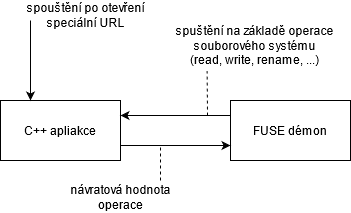
\includegraphics[width=0.55\linewidth]{other-fig/architecture.png}
    \caption{Vysokoúrovňový návrh architektury aplikace.}
\end{figure*}

Pokud FUSE démon má vykonat akci, pro kterou nemá dostatečné informace, spustí jako další subproces druhou hlavní aplikaci a počká na návratovou hodnotu, na základě
které se rozhodne, jakým způsobem onu akci dokončí. Může se jednat o situace jako: je soubor určený jen pro četní nebo i zápis, je daný soubor stále validní
(nevypršel datum expirace) apod.

V této variantě je FUSE démon velmi minimalistický a zbytek funkcionality je implementován v druhé aplikaci, která běží jen pokud je k tomu vyzvaná, narozdíl od neustále
běžícího démona. Démon tedy po celou dobu běhu zabírá méně místa, protože nemusí mít načtené v paměti všechny potřebné knihovny. Na druhou stranu mohou být tyto knihovny
i tak namapované, protože je můžou využívat jiné aplikace. Démon musí být spuštěný s oprávněními superuživatele \texttt{root} a menší množství kódu běžícího s vysokými
oprávněními implikuje menší náchylnost na bezpečnostní chyby. Hlavní aplikace může běžet jen s právy přihlášeného uživatele, což je jedna z dalších výhod oproti 
druhé zvažované variantě.

\subsection{Diagram tříd}

Aby implementace probíhala s možná nejmenším množstvím komplikací a nebylo třeba již uvažovat nad dalšími rozhodnutími, byl vytvořen diagram tříd \ref{fig:class_diagram_design},
který se pokouší podrobně vizualizovat třídy s atributy a metodami, jež je třeba implementovat. Jedná se pouze o návrh, který se v průběhu vývoje bude měnit, ale pokud je návrh
kvalitní a vývojáři se jej snaží dodržet, neměl by být výsledek zásadně rozdílný.

\begin{figure*}[h]
    \centering
    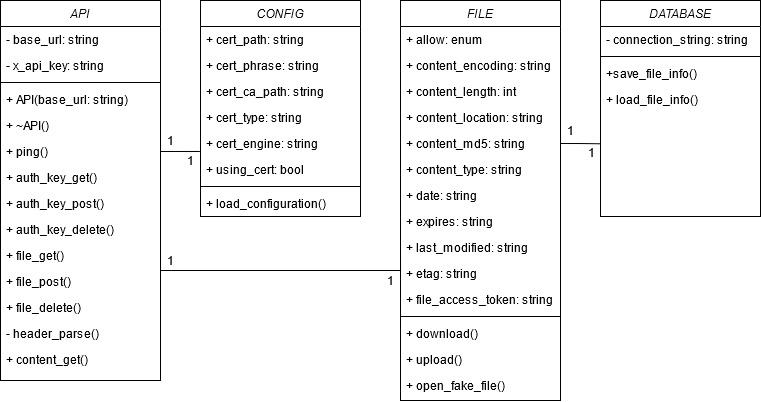
\includegraphics[width=1\linewidth]{other-fig/class_diagram_design.png}
    \caption{Diagram tříd - návrh.}
    \label{fig:class_diagram_design}
\end{figure*}

Na obrázku \ref{fig:class_diagram_implementation} je možné vidět diagram tříd naimplementovaného programu. Na první pohled vypadá velmi rozdílně, po bližším prozkoumáním
lze vidět jednu novou třídu oproti návrhu. Jedná se o třídu zobrazující notifikace pro uživatele, která nemá vliv na hlavní funkcionalitu. Dále přibylo několik podpůrných
funkcí a také přibily některé atributy, případně se přejmenovaly. Při implementaci nenastaly žádné zásadní potíže způsobené chybným nebo nepřesným návrhem, tudíž lze
návrh označit za úspěšný.

\newpage

\begin{figure*}[h]
    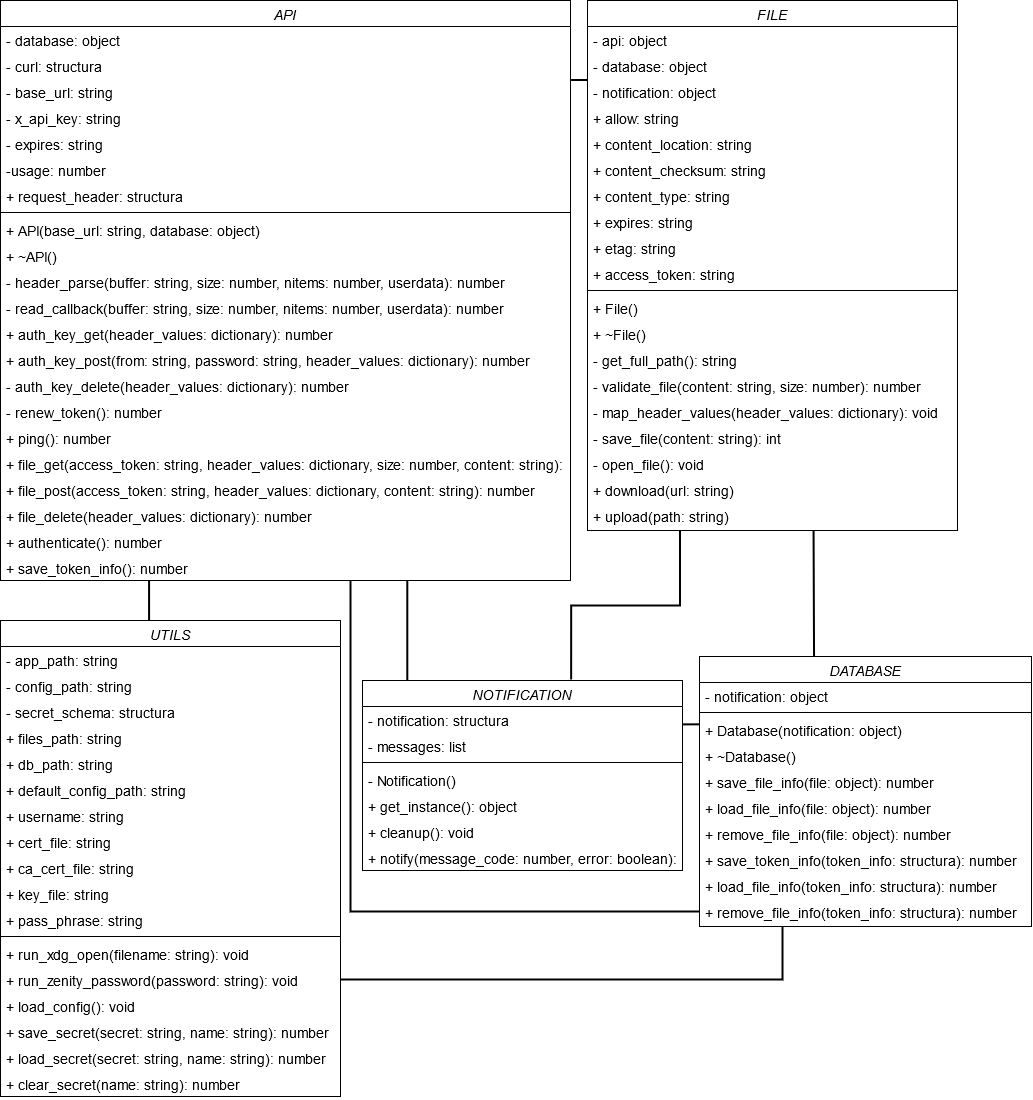
\includegraphics[width=1\linewidth]{other-fig/class_diagram_after_implementation.png}
    \caption{Diagram tříd - téměř hotová implementace.}
    \label{fig:class_diagram_implementation}
\end{figure*}

\section{Technologie}

V této sekci budou popsány jednotlivé technologie, které ovlivnily tuto práci. Pro samotný návrh stačí elementární znalosti daných technologií, ale pro
implementaci a jejich správné a efektivní využití je třeba jejich bližší pochopení. Za klíčovou technologii by se dala označit technologie FUSE, bez které
by řešení nemohlo splňovat zadaná kritéria.

\subsection{GNU/Linux}

GNU je rekurzivní zkratka pro „GNU's Not Unix!“. Jedná se o projekt, který měl za cíl vystavět nový operační systém kompatibilní s Unixem. Všechen kód vytvořený pod
tímto projektem je tzv. free software (svobodný software). Jedná se o filosofii vývoje software jejíž parafrázovaná definice je následující. Svobodný (free) software se
vztahuje ke svobodě, ne k ceně. Slovo svobodný (free) by mělo být bráno ve významu svobodný projev (free speech) nikoliv pivo zdarma (free beer) \cite{FreeSoftware}.

V projektu GNU postupně vznikaly jednotlivé softwarové balíky, které měly ve výsledku poskládat nový operační systém. Pod projektem GNU vnikli aplikace jako překladač GCC,
textový formátovač TeX, terminálový shell Bash a mnohé další. Na počátku 90. let byl systém téměř hotový, scházelo jen jádro operačního systému. Ve stejném období dokončoval
Linus Torvalds své jádro operačního systému nazývané Linux. \cite{GNULinux} \cite{GNULinux2} 

Vznikla tedy myšlenka tyto dva projekty spojit a po vyřešení problémů s kompatibilitou jednotlivých částí projektů vnikl GNU/Linux. Balíčky projektu GNU umožnovaly práci
se systémem postaveným nad Linuxovým jádrem. Všechny dnešní distribuce jako jsou Debian, Fedora a další jsou distribuce systému GNU/Linux. Linux je název pouze jádra pro 
operační systém, který zevšeobecněl a je tímto názvem chybně označován celý systém. Projekt GNU dodnes vyvíjí své jádro pojmenované GNU Hurd, se kterým by vznikl operační
systém GNU, což byl počáteční cíl projektu. \cite{GNULinux2}

\begin{figure*}[h]
    \centering
    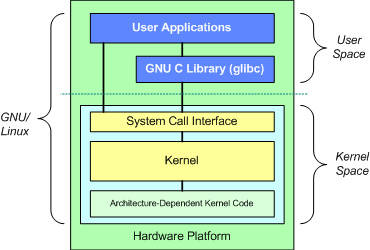
\includegraphics[width=0.6\linewidth]{other-fig/userspace.jpg}
    \caption{Architektura GNU/Linux. Převzato z \cite{Userspace}.}
    \label{fig:gnu_linux_architecture}
\end{figure*}

Architekturu GNU/Linux vyobrazená na obrázku \ref{fig:gnu_linux_architecture} vyznačuje hranici mezi kernelem a uživatelským prostorem. Jádro/kernel běží v tzv. priviligovaném
režimu, což je režim s nejvyššími oprávněním a může na CPU provádět jakékoliv operace. Všechny ostatní aplikace běží v uživatelském prostoru a jsou omezeny jen na provádění 
podmnožiny operací oproti priviligovanému režimu. Pokud aplikace potřebuje vykonat operaci, která vyžaduje vyšší oprávnění, zažádá jádro operačního systému, aby tuto operaci 
provedlo místo ní. Tím je docíleno vyššího zabezpečení operačního systému.

\subsection*{Desktopová prostředí}

V GNU/Linxovém prostředí existuje velké množství desktopových prostředí. Každé z nich je založeno na tzv. display serveru. Jedná se o program zodpovědný za koordinaci
komunikace mezi grafickým prostředím a kernelem. Se svými klienty komunikuje pomocí proprietárního protokolu. V GNU/Linux systémech jsou dnes rozšířené dva display servery
X.org a Wayland. Wayland je novější implementací display serveru a postupně v jednotlivých distribucích nahrazuje X.Org.

Každé desktopové rozhraní je něčím specifickým a vývoj software schopný běžet na všech desktopových rozhraních může vyžadovat větší úsilí. Mezi běžně používaná desktopová 
rozhraní patří například GNOME, KDE, Xfce, MATE a mnohé další.

\subsection{C++/C}

Jazyk C patří do skupiny dlouho používaných programovacích jazyků. Se svou bohatou historií sahající až do 70. let 20. století velmi ovlivnil další nástupnické procedurální
jazyky jako C++, C\#, Java atd. V roce 1989 byl jazyk standardizován jako ANSI C a následně přišly ISO standardy označované jako C99, C11, C17. Jazyk C je řazen mezi
vysokoúrovňové programovací jazyky, přestože je relativně jednoduchý a obsahuje malé množství konstrukcí v porovnání s ostatními jazyky.\cite{CReference}

Vývoj C++ je oproti C dynamičtější, což můžeme vidět na jednotlivých ISO standardech C++98, C++03, C++11, C++14, C++17 a C++20. Jazyk C++ se v poslední dekádě velmi
proměnil a období od standardu C++11 je označováno za dobu „moderního C++“. V posledním standardu přibyla například podpora konceptů nebo rozsahů.\cite{CPPReference}

Při využití překladačů GCC nebo G++ lze využít tzv. GNU rozšiřující standardy. Poté je možné využít některé konstrukce, které nejsou specifikované v oficiálním ISO standardu.
V případě jazyka C se jedná o standardy pojmenované GNU99, GNU11 a GNU17, v případě C++ se jedná o GNU++11 a jemu podobné.

\subsection{HTTP}

Hypertext Transfer Protokol je protokol aplikační vrstvy TCP/IP stacku. Byl vytvořen pro přenášení hypertextových souborů v 90. letech 20. století a dnes se jedná o nejrozšířenější
aplikační protokol. Poslední stabilní verze protokolu označená jako HTTP/2 byla vydaná v roce 2015. Aktuálně je ve fázi specifikace nástupce pojmenovaný HTTP/3.

HTTP v čisté formě dnes již téměř není možné potkat, ale využívá se ve spojení s šifrovacím protokolem TLS. Při komunikaci se nejprve vytvoří TCP spojení a poté šifrovaný kanál,
skrze který je HTTP bezpečně přenášeno. Toto řešení není nejefektivnější, protože vznikalo postupně a spojovaly se technologie, které nebyly od počátku navržené pro tento účel.
Ve většině případů uživatel na stabilním připojení nezaregistruje žádné potíže, kterými tyto technologie trpí. Jedním z problémů je dlouhá časová prodleva, než se kanál ustálí
pro přenášení dat. Tento problém má vyřešit právě nová verze HTTP. \cite{HTTP3}

\begin{figure*}[h]
    \centering
    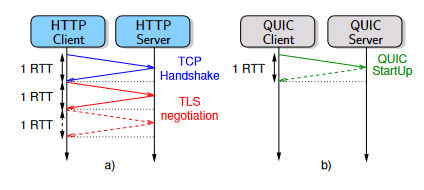
\includegraphics[width=0.8\linewidth]{other-fig/http_comparison.png}
    \caption{Porovnání HTTP verze 2 (a) a 3 (b). Převzato z \cite{HTTP3}.}
    \label{fig:http_comparison}
\end{figure*}

Nová verze využívá nový protokol QUIC, který je přenášen protokolem UDP namísto TCP jako tomu bylo u předchozích verzích HTTP. Na obrázku \ref{fig:http_comparison}
je možné vidět, že navázání komunikace je ze tří výměn informací zredukováno jen na jednu. Formát hlavičky HTTP by měl zůstat nezměněný, a tudíž je zpětně kompatibilní.

Pro tento projekt je důležitá práce s datumy, přesněji formáty umožněné přenášet ve validní HTTP hlavičce. RFC7231 specifikuje tři formáty datumů, z nichž dva
jsou označené jako zastaralé, ale jsou stále validní. Udržované jsou kvůli zpětné kompatibilitě s protokolem HTTP/1.1. \cite{RFC7231}

\begin{itemize}
    \item Upřednostňovaný formát
    \begin{itemize}
        \item Sun, 06 Nov 1994 08:49:37 GMT (IMF-fixdate formát)
    \end{itemize}
    \item Zastaralé formáty
    \begin{itemize}
        \item Sunday, 06-Nov-94 08:49:37 GMT (RFC 850 formát)
        \item Sun Nov  6 08:49:37 1994 (ANSI C asctime() formát)
    \end{itemize}
\end{itemize}

\subsection{OpenAPI}

Jedná se o standard pro definování metod REST API, který má v čase psaní této práce poslední verzi 3.0.3. Zápis je možný ve dvou jazycích: JSON a YAML. Oba 
je možné strojově zpracovat, a přitom jsou pro člověka stále čitelné. 

Specifikace je velmi obsáhlá a umožňuje popsat API velmi detailně a přitom efektivně. Například je možné vytvářet šablony datových struktur, které jsou používány jako
vstupní, nebo naopak návratové hodnoty jednotlivých funkcí. V definici je pak možné na tuto šablonu odkázat. Struktura souboru je hierarchická a skládá se z jednotlivých objektů.
Každý objekt má povinné a volitelné atributy. Definovat tedy lze hlavičky požadavku, URL query parametry, návratové kódy a k nim přiřazené hlavičky odpovědí a odpovědi samotné,
případně příklady možných odpovědí. Toto je jen stručný výpis možností, které standard OpenAPI definuje. \cite{OpenAPI}

\subsection{Mock Server}

Mock Server je speciální případ testovacího vzoru Mock Object, který spadá do kategorie Test Double. Test Double je kategorie testovacích vzorů, do které patří
vzory jako právě Mock Object, Fake Object, Test Stub apod. Jednotlivé vzory mohou být mezi sebou zaměnitelné, protože jejich definice a použití je velmi podobné. 
Tato kategorie vrozů je využívaná pro systémy, které pracují s určitou externí komponentou, která není dostupná nebo by testování ovlivnila svými nežádoucími
vedlejšími účinky.\cite[522--524]{UnitPatternsTest} K využití Mock Serveru bylo přistoupeno z důvodu nedostupnosti VDU, při vzniku této práce. Mock Server nebyl využíván 
jen pro účely testování, ale i během vývojové fáze. Aby nedošlo k zanesení chyby do software během vývoje, byla napsána sada testů, která ověřovala správnou
implementaci Mock Serveru vůči předem specifikované definici.

\begin{figure*}[h]
    \centering
    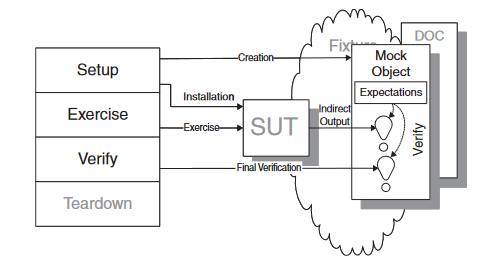
\includegraphics[width=0.67\linewidth]{other-fig/mock_object.png}
    \caption{Test Double schéma. Převzato z \cite[544]{UnitPatternsTest}.}
\end{figure*}

Mock Object pokrývá funkcionalitu Test Stub vzoru a na vývojáři záleží, jakým způsobem využije tyto možnosti. V kontextu této práce by se používaný Mock Server dal
klasifikovat jako pouhý Test Stub, protože není využívaná verifikující část, kterou definuje Mock Object vzor. \cite[524--525]{UnitPatternsTest} Verifikovaný je pouze
výstup funkcí v testovaném systému.

\subsection{Souborový systém v uživatelském prostoru (FUSE)}
\label{sec:fuse}

FUSE je označení pro File system in userspace a jedná se o framework umožňující vytvořit vlastní virtuální souborový systém v uživatelském prostoru. FUSE se skládá
ze dvou částí, démona a modulu pro jádro operačního systému. Je-li modul načtený registruje ovladač v Linuxovém VFS (Virtual filesystem). Tento ovladač poté
představuje proxy pro všechny běžící démony. FUSE driver obsahuje několik front pro obsloužení všech potřebných akcí. Nejprioritnější fronta je pro obsloužení
přerušení, ostatní fronty jsou pro obsluhu synchronních, asynchronních a a tvz. forget požadavků. Priorita zpracování těchto front je daná poměrem 8 ku 16 pro 
synchronní a asynchronní ku forget požadavkům. \cite{FuseOrNotToFuse}

\begin{figure*}[h]
    \begin{subfigure}[h]{.45\linewidth}
        \centering
        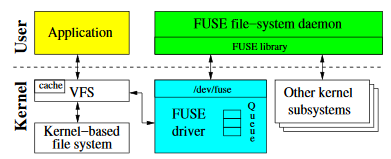
\includegraphics[width=1 \linewidth]{other-fig/FUSE_architecture.png}
        \caption{Architektura. Převzato z \cite{FuseOrNotToFuse}.}
    \end{subfigure}
    \hfill
    \begin{subfigure}[h]{.45\linewidth}
        \centering
        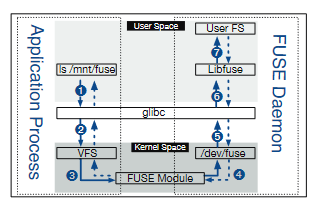
\includegraphics[width=1 \linewidth]{other-fig/FUSE_dataflow.png}
        \caption{Datový tok. Převzato z \cite{HardeningFUSE}.}
        \label{fig:fuse_dataflow}
    \end{subfigure}
    \caption{Vysokoúrovňové diagramy architketury a datového toku pro FUSE}
\end{figure*}

Démon zpracovává postupně požadavky, které se přidávají do front ve FUSE ovladači. Na obrázku \ref{fig:fuse_dataflow} je vidět, jak požadavek prochází jednotlivými částmi
systému. Aplikace přistoupí na připojený FUSE souborový systém a požadavek projde skrze VFS a FUSE ovladač až k démonovi. Démon daný požadavek zpracuje, ve většině případů
přistoupí na hostitelský souborový systém a vykoná na něm požadovanou operaci. Odpověď je poté navrácena stejným způsobem, jakým byla přenesena k FUSE démonovi.

Démon nemusí implementovat všechny operace, záleží jen na požadavcích. Je-li potřeba vytvořit souborový systém jen pro čtení, implementují se například operace
INIT, OPEN, GETATTR, READ a RELEASE. Mohou být implementované další kvůli optimalizacím, nebo řešící specifické případy. Více informací k jednotlivým operacím
je možné dohledat v dokumentaci libfuse\footnote{\url{http://libfuse.github.io/doxygen/structfuse__operations.html}}.

\begin{table}[h]
    \begin{center}
        \begin{tabularx}{14cm}{|l|X|} 
            \hline
            \textbf{Skupina} & \textbf{Typ požadavku} \\
            \hline
            Speciální & INIT, DESTROY, INTERRUPT \\
            \hline
            Metadata & LOOKUP, FORGET, BATCHFORGET, CREATE, UNLINK, LINK, RENAME, RE-NAME2, OPEN, RELEASE, STATFS, FSYNC, FLUSH, ACCESS \\
            \hline
            Data & READ, WRITE \\
            \hline
            Atributy & GETATTR, SETATTR \\
            \hline
            Rozšířené atributy & SETXATTR, GETXATTR, LISTXATTR, REMOVEXATTR \\
            \hline
            Symbolické linky & SYMLINK, READLINK \\
            \hline
            Složky & MKDIR, RMDIR, OPENDIR, RE-LEASEDIR, READDIR, READDIRPLUS, FSYNCDIR \\
            \hline
            Zamikání & GETLK, SETLK, SETLKW \\
            \hline
            Misc & BMAP, FALLOCATE, MKNOD, IOCTL, POLL, NOTIFYREPLY \\
            \hline
        \end{tabularx}
        \caption{Tabulka typů poždavku pro zpracování FUSE démonem. Převzato z \cite{FuseOrNotToFuse}.}
    \end{center}
\end{table}

\subsection{D-Bus}

D-Bus je systém pro posílání zpráv mezi jednotlivými aplikacemi. Přesněji se jedná o Inter-Process Communication (IPC) a Remote Procedur Calling (RPC) mechanismus
vytvořený pro komunikaci mezi jednotlivými procesy na stejném počítači. D-Bus funguje na Unix-like systémech a port pro operační systém Windows je také dostupný.
Existuje také reimplementace D-Bus protokolu pro další jazyka jako je Java, C\# nebo Ruby. Objekty jsou identifikovány kombinací tzv. „bus name“ a „object path“. \cite{DBus}

Existují dva typy „bus name“, jeden je unikátní a je přiřazen každé připojené aplikaci na sběrnici. Pro tyto unikátní jména lze vytvořit alias nazývaný jako
„well-known bus name“. Například pro přístup ke keyringu je používaný alias „org.freedesktop.secret“. „Object path“ poté identifikuje danou funkci zpřístupněnou 
pro D-Bus. Komunikace klienta s danou službou poté funguje velmi podobně jako zjišťování IP adresy z doménového jména pomocí DNS. Klient započne komunikaci dotazem
na přeložení „well-known bus name“. V odpovědi dostane unikátní „bus name“, který může využít pro komunikaci s cílovým procesem. \cite{DBus}

\subsection{Keyring}

Pro ukládání hesel nebo tokenů pro aktuálně přihlášeného uživatele v systému lze využít službu pojmenovanou keyring. Podle implementace se heslo uloží na disk,
nebo je jen načtené v operační paměti. Pokud je uživatel přihlášený, je mu heslo k dispozici, při vypnutí systému nebo odhlášení uživatele je heslo z operační paměti
odstraněno. Ukládá-li se heslo na disk, je zašifrováno a odšifrovat ho může jen uživatel, který heslo do keyringu uložil. Pokud není heslo k dispozici musí jej aplikace 
od uživatele vyžádat a do keyringu případně uložit. Pokud aplikace využívající keyring nemusí s uživatelem tolik interagovat a práce bývá pro uživatele příjemnější,
přitom heslo je velmi dobře chráněno. Utočník napadající systém z vnějšku není schopen heslo zjistit bez jeho dešifrování. \cite{Keyring}

GNU/Linux obsahuje keyring aplikaci pojmenovanou linux-keyring. Některá desktopová prostředí obsahují své keyring aplikace, které rozšiřují možnosti základního linux-keyringu.
Například desktopové prostředí GNOME obsahuje aplikaci gnome-keyring a desktopové prostředí KDE zase aplikaci kde-wallet. \cite{Keyring}

% ---------------------------------------------------------------------------------------------------------------------------------------
\chapter{Popis implementace a nasazení aplikace}

Při vývoji byly využity kromě standardních knihoven jazyka C a C++ také knihovny umožňující práci s databází, notifikování uživatele pomocí 
systémového notifikačního systému nebo knihovna pro vytvoření automatizovaných testů.

\begin{itemize}
    \item \textbf{libcurl} – Knihovna pro jednoduché přenášení dat po síti. Podporuje velkou řadu protokolů jako FTP, HTTP, IMAP atd. Šifrování je zpřístupněno pomocí
    externí knihovny (např. openssl). V posledních verzích knihovny je možné pracovat s draft verzí protokolu HTTP verze 3. \cite{libcurl}
    \item \textbf{libnotify} – Jedná se o implementaci Desktop Notification Specification\footnote{\url{https://developer.gnome.org/notification-spec/}}, který specifikuje
    jednotné rozhraní pro vytváření notifikací v desktopových prostředích. Pro korektní využití libnotify je třeba mít běžící notifikační server, se kterým se komunikuje
    pomocí D-Bus. Většina desktopových prostředí má vlastní implementaci notifikačního serveru startující při spuštění systému. \cite{libnotify}
    \item \textbf{libfuse} – Nabízí funkce pro vytvoření FUSE démona, komunikující s FUSE modulem kernelu. Implementací jednotilivých operací je možné vytvořit vlastní
    souborový systém v uživatelském prostoru. \cite{libfuse}
    \item \textbf{libsqlite3} – Knihovna pro práci s jednosouborovou databází SQLite. Jedná se o malou samostatnou a nejpoužívanější databázi na světě. Interakce s databází
    je vedena v jazyku SQL. Zajímavost týkající se SQLite je plán podpory a udržování do roku 2050. \cite{libsqlite}
    \item \textbf{libssl} – Šifrovací knihovna pro obecné použití, ale s primárním zaměřením na protokoly TLS a SSL. V této práci byla použita jen pro výpočet kontrolního
    součtu algoritmem MD5. \cite{libssl}
    \item \textbf{libsecret} – Se službou keyring je možné komunikovat pomocí D-Bus sběrnice. Knihovna libsecret zapouzdřuje tuto komunikaci do svého API a vytváří tak
    jednoduše použitelné rozhraní. \cite{libsecret}
    \item \textbf{libgtest} – Google Test je testovací framework pro psaní jednotkových testů pro programy psané v jazyce C++. Je založen na architektuře xUnit. Zpřístupňuje
    makra pro ověření výroku nebo podmínky je-li pravdivá. \cite{libgtest}
\end{itemize}

\noindent Další balíčky využité při vývoji nebo jsou potřeba pro běh aplikace samotné.

\begin{itemize}
    \item \textbf{Zenity} – Aplikace pro vytváření jednoduchých dialogových oken.
    \item \textbf{DB Browser for SQLite} neboli \textbf{sqlitebrowser} - Grafický prohlížeč SQLite databází, umožňující zobrazení obsahu tabulek, vytvoření i úpravu dat
    nebo struktury databáze.
    \item \textbf{Behave} – Software pro psaní testů v přirozeném jazyce. Je využíván pro automatické testování software.
    \item \textbf{Doxygen} – Nástroj pro generování dokumentace z anotací v kódu. Dokumentace může být ve formátu PDF dokumentu nebo HTML souborů.
\end{itemize}

\section{Využívané cesty v Linuxové adresářové struktuře}

Linuxová hierarchie má své konvence, kde by se jednotlivé soubory měly nacházet. Také existuje specifikace nazývaná XDG Base Directory specification\footnote{\url{https://specifications.freedesktop.org/basedir-spec/basedir-spec-latest.html}},
která řeší například ukládání aplikačních dat pro jednotlivé uživatele. Tím je myšleno, že každý uživatel může mít vlastní konfiguraci aplikace. V tomto případě proto není
možné používat globální složky vytvořené k tomuto účelu (např. \texttt{/var}). Některé z použitých souborů nebo složek mají název začínající tečkou, jedná se o skryté
soubory/složky. Znalý uživatel si tyto složky může ve svém průzkumníku souborů zobrazit a jednoduše k nim přistoupit.

Aplikace je nastavena a byla pro tento případ i vyvíjena, že každý uživatel má vlastní konfiguraci a také ve FUSE souborovém systému vidí pouze své soubory. Toto řešení
působilo při vývoji velké potíže, protože FUSE démon musí být spouštěn s právy superuživatele \texttt{root} a tím pádem nemůže použít proměnnou \texttt{\$HOME}. Bohužel 
totiž neukazuje do domovského adresáře přihlášeného uživatele, ale do domovského adresáře superuživatele \texttt{root}.

Po podrobném znovu přečtení dokumentace k FUSE technologii se objevila jedna možnost, jak tento problém vyřešit. V dokumentaci však nebyl tento případ dobře rozveden, ale 
finální řešení bylo, že binární soubor reprezentující FUSE démona musel mít nastaveného vlastníka uživatele \texttt{root} a také tomuto souboru musel být nastaven 
tzv. suid bit. Díky tomuto nastavení může FUSE démon běžet pod přihlášeným uživatelem, avšak s oprávněními speruživatele \texttt{root}.
\\\\
\noindent Seznam souborů a cest využívaných aplikací:

\begin{itemize}
    \item \textbf{/usr/local/bin} – Místo pro programy neboli spustitelné soubory, přístupný pro normálního uživatele. \cite{LinuxHierarchy} V této složce jsou uloženy
    oba binární soubory pojmenované \texttt{vdu-app} a \texttt{vdu-app-fuse}. Druhá jmenovaná je FUSE démon, který musí mít vlastníka uživatele \texttt{root} a nastavený
    tzv. suid bit. Aplikace \texttt{vdu-app} nevyžaduje žádné specifické požadavky. 
    \item \textbf{/mnt/vdu} – Složka \texttt{/mnt} je určená pro připojování (mount) externích paměťových zařízení jako USB flash disk, CD apod. nebo pro připojení
    sídílené slokžy nebo síťového disku. Do této složky bude připojen FUSE souborový systém, který bude využíván pro ukládání stažených souborů z VDU.
    \item \textbf{\$HOME/.local/share/vdu/} – Na této cestě budou umístěny aplikační data jako databáze a složka pro ukládání obsahu z FUSE souborového systému.
    Každému uživateli, který bude na daném operačním systému využívat \texttt{vdu-app} bude vytvořena tato složka.
    \begin{itemize}
        \item \textbf{/vdu.db} – SQLite 3 databáze pro ukládání podpůrných informací o souborech stažených z VDU a také metadata potřebná pro běh programu.
        \item \textbf{/fuse} – Složka na hostitelském souborovém systému, kterou využívá FUSE démon pro čtení a ukládání dat, která jsou následně zobrazena
        ve složce \texttt{/mnt/vdu}. Pokud by uživatel chtěl obejít FUSE souborový systém, mohl by k datům přistoupit napřímo skrze tuto složku. Poté by mohl
        číst soubory, které již expirovali, nebo zapisovat do souborů, ke kterým má pouze práva na čtení. Vlastník této složky je \texttt{root}, který jako
        jediný může z této složky číst nebo do ní zapisovat. Jak již bylo výše popsáno FUSE démon běží s právy superuživatel \texttt{root}, takže může nad tomuto
        složkou operovat.
    \end{itemize}
    \item \textbf{\$HOME/.vdu.conf} – Konfigurační soubor aplikace, který je také pro každého uživatele jedinečný.
    \item \textbf{/usr/share/applications} – Složka pro ukládání tzv. Desktop Entries, což jsou soubory definující aplikace, které mají být určitým způsobem integrovány
    do desktopového prostředí. Desktop Entry obsahuje údaje jako jméno, ikonu, popis, přiřazený typ souboru atd. \cite{DesktopEntrySpecification}
    \item \textbf{/etc/systemd/user} – Konfigurační složky systému \texttt{systemd}, využívané pro definici jednotlivých systemd služeb (systemd service). V tomto 
    případě pro služby běžící pro každého jednotlivého přihlášeného uživatele. Systémová služba by byla umístěná namísto složky \texttt{user} ve složce \texttt{system}. \cite{systemd-user}
\end{itemize}

\subsection{Konfigurační soubor}
\label{subsec:config}

Jedná se o textový sobor obsahující dvojice klíč a hodnota oddělené znakem rovnítka. Každá tato dvojice musí být na samostatném řádku. Prázdné řádky nebo řádky
začínající znakem „\#“ jsou přeskakovány. Jedná se o standartní pojetí konfiguračního souboru na systému GNU/Linux.

\begin{lstlisting}[caption={Příklad obsahu konfiguračního souboru.}]
Username = username
ClientCertFile = client.pem
CACertFile = ca.pem
KeyFile = client.key
#Passphrase = SuperSecretPassPhraseXX12@
\end{lstlisting}

Konfigurační soubor umožňuje nastavit uživatelské jméno, jména certifikátů nebo klíčů a v neposlední řadě také volitelnou frázi pro zabezpečení certifikátu.
Všechny hodnoty jsou volitelné neboli pokud nebudou v konfiguračním souboru nastavené, aplikace zvolí jejich výchozí hodnotu. Případně vyzve uživatele pro doplnění
informací, které jsou třeba pro správné fungování.

Pokud není nastaveno uživatelské jméno, tak výchozí hodnotou je uživatelské jméno z operačního systému. Pro certifikáty je situace podobná, nejsou-li nastavené
všechny hodnoty jako jméno klientského certifikátu, jméno certifikátu certifikační autority a jméno souboru obsahující privátní klíč, tak je využita autentifikace přes
heslo. Bezpečnostní fráze je volitelná, protože ne každý certifikát musí být touto frází zabezpečený. Nezadává se absolutní cesta k certifikátům, ale pouze jejich jméno,
protože certifikáty jsou následně načítány z systémového uložiště certifikátů.

\subsection{SQLite databáze}

Hlavní vyvíjená aplikace potřebuje uchovávat data mezi jednotlivými běhy a SQLite databáze je pro tento případ asi nejvhodnější metoda. Jedná se o jednosouborovou databázi,
která zapouzdřuje kompletní SQL engine. Databáze obsahuje dvě tabulky a to \texttt{Files} a \texttt{Metadata}. Databáze se vytváří automaticky pokud se na dané cestě nenachází.

V tabulce \texttt{Files} jsou udržovány informace o jednotlivých souborech, které se právě nacházejí na FUSE souborovém systému. Tabulka \texttt{Metadata} má pouze dva
sloupce a funguje pro ukládání dvojic klíč a hodnota stejného typu. Taková tabulka by se dala přirovnat slovníku v programovacím jazyce Python nebo C\#. C++ ekvivalent by
byl kontejner \texttt{std::map}. Využívat tabulku takovým způsobem není konvenční, ale nezatěžuje to vývoj projektu dalším odlišným způsobem ukládání dat 
(např. do strukturovaného souboru).

\begin{figure*}[h]
    \centering
    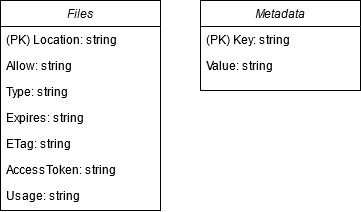
\includegraphics[width=0.6\linewidth]{other-fig/database.png}
    \caption{Schéma SQLite databáze.}
\end{figure*}

Pokud SQL dotaz obsahuje parametry, využívá se postup před vytvoření dotazu bez parametrů a jejich následné navázání na již zkompilovaný dotaz. Tento postup by měl zabránit
technice napadení databázového systému nazývané SQL injection. K tomuto účelu obsahuje libsqlite3 sadu funkcí jako \texttt{sqlite3\_prepare}, \texttt{sqlite3\_bind},
\texttt{sqlite3\_column}. \cite{sqlite-c} Veškerá komunikace s databází je zapouzdřená ve třídě \texttt{Database}.

\section{xdg-utils}
Projekt xdg-utils je soubor nástrojů a shell scriptů, který se snaží vytvořit jednotné rozhraní pro práci na různých desktopových prostředích. Asi polovina nástrojů se 
zaměřuje na proces instalace aplikace a druhá polovina se zase věnuje integraci aplikací do desktopového prostředí. Integrace spočívá ve využívání instalovaných aplikací
desktopovým prostředím jako otevření souboru ve specifické aplikaci nebo přiřazení ikony pro určitý typu souborů.

Dále se budeme zabývat jen nástroji \texttt{xdg-mime} a \texttt{xdg-open}, které jsou v rámci této práce využívané. Xdg-open zajišťuje otevření určité URL nebo typu souboru
v přiřazené aplikaci. Přiřazovat lze pouze k aplikacím popsaných tzv. Desktop Entries, které jsou specifikové v Desktop Entry Specification\footnote{\url{https://specifications.freedesktop.org/desktop-entry-spec/latest/}}.
Specifikace také definuje vestavěné proměnné pro předávání cesty k souboru nebo vyhledávané URL. Příkaz xdg-open je volán v případě, že je potřeba uživateli otevřít soubor ve
správné aplikaci po stažení souboru z VDU. \cite{xdg}

\begin{lstlisting}[caption={Příklad struktury Desktop Entry souboru.}]
[Desktop Entry]
Type=Application
Version=1.0
Name=VDU App
Comment=Application for handling remote VDU files in desktop enviroment
Exec=/usr/local/bin/vdu-app --url-handler %u
MimeType=x-scheme-handler/vdu;    
\end{lstlisting}

Druhý nástroj xdg-mime umožňuje vytvořit nový MIME type nebo přiřadit k určitému MIME typu Desktop Entry aplikaci. Také umí vyhledávat jaké Desktop Entries jsou přiřazené
k určitému MIME typu nebo k jakému MIME typu je přiřazena daná Desktop Entry. Pro registraci speciálního URL protokolu se využívá MIME type pojmenovaný 
\texttt{\mbox{x-scheme-handler/<název protokolu>}}. \cite{xdg}

\section{Komunikace s API}

Pro komunikaci s VDU skrze protokol HTTP byla vybrána knihovna libcurl pocházející z projektu cURL vyvíjející stejně pojmenovaný nástroj. Knihovna může provádět
synchronní i asynchronní volání na základě zvoleného rozhraní. Při vývoji bylo využito tzv. Easy rozhraní umožňující pouze synchronní volání. Využití asynchronního volání
nedávalo smysl, protože by aplikace neměla v daném mezičase co vykonávat. Všechny API volání definované externím zadavatelem byly implementované ve třídě pojmenované API.

Metoda pro zneplatnění autentifikačního tokenu (DELETE /auth/key) nebyla jako jediná využita, protože aplikace implementuje vlastní způsob zneplatnění tohoto tokenu. Blíže 
je tato implementace popsaná v podsekci \ref{subsec:authentication}.

\subsection{Mock Server}

Pro implementaci Mock Serveru byla vybrána aplikace Postman. Bohužel to nebyla úplně nejlepší volba. Nedostatky tohoto řešení byly lehce limitující, ale až v pozdnějších
fázích vývoje projektu a hledat nové řešení postrádalo význam. Jiné řešení by mohlo trpět jinými nedostatky, a proto bylo zvolen kompromis.

Aplikace Postman totiž využívá některé HTTP hlavičky požadavku pro identifikaci nebo rozhodování, jak naložit s daným voláním. Při využití hlavičky \texttt{x-api-key}, která
podle specifikace API VDU má obsahovat autentifikační token. Aplikace Postman toto pole využívá pro ověření přístupu k privátním Mock Serverům. Aby využívaný
Mock Server mohl zůstat veřejný, přejmenovalo se pole \texttt{x-api-key} na \texttt{x-api-key-test}. Toto nastavení muselo být řešeno na úrovni kódu, a proto byly do aplikace 
přidané direktivy preprocesoru pro podmíněný překlad. Pokud je definovaný symbol \texttt{VDU\_DEV}, tak je využíváno jméno hlavičky s koncovkou test.

Definovaný je ještě jeden symbol \texttt{VDU\_HTTP\_3}, který v knihovně libcurl vynucuje využití protokolu HTTP/3. Tuto funkcionalitu nebylo možné otestovat, protože aplikace
Postman tento protokol ještě nepodporuje. Jedná se však o možnost dalšího rozvoje, který je třeba pouze otestovat a odladit případné nedostatky a chyby.

\subsection{Autentifikace}
\label{subsec:authentication}

VDU umožňuje autentifikovat uživatele pomocí uživatelského jména a hesla, nebo uživatelského jména a klientského certifikátu. Jak bylo zmíněno v podsekci \ref{subsec:config}
tak uživatelské jméno je možné nastavit v konfiguračním souboru, nebo je jako výchozí hodnota použito jméno z operačního systému.

Při využívání hesla je uživatel poprvé dotázán za pomocí aplikace Zenity, aby zadal své heslo. Aplikace poté zadané heslo uloží do keyring aplikace a je-li potřeba znovu ověřit
uživatelovu identitu je heslo vyhledáno v keyring aplikaci a automaticky využito pro tuto akci. Pokud se nejedná o keyring aplikaci ukládající data perzistentně nebo je
heslo manuálně odebráno, tak je uživatel při nemožnosti heslo vyhledat znovu vyzván k zadání hesla.

Využití certifikátů je pro uživatele pohodlnější možností, protože nenastane situace, na kterou by musel uživatel přímo reagovat a vše se děje automaticky. Pro využití
certifikátů je třeba klientský certifikát, tak i certifikát certifikační autority nainstalovat do systému pomocí nástrojů specifických pro danou distribuci. Jsou-li certifikáty
nainstalované, poté stačí nastavit v konfiguračním souboru korektně hodnoty a identita uživatele je následně ověřena za pomoci klientského certifikátu.

Poté co je uživatel ověřen aplikace obdrží od VDU token, který se uloží také do keyring aplikace pro případné znovupoužití. Informace o tokenu jsou uloženy do 
tabulky \texttt{Metadata} v databázi. Jedná se přesněji o datum expirace a počet dalších použití. Aplikace má totiž implementovanou funkcionalita, že každý autentifikační token
může být využit maximálně 5krát. Pokud má být token použit po šesté, tak je místo toho zavolaná funkce pro výměnu tokenu a nový navrácený token je použit namísto starého.

\section{FUSE démon}

Démon připojuje obsah složky \texttt{\$HOME/.local/share/vdu/} do \texttt{/mnt/vdu} a pokud v připojeném bodu nastane nějaké akce řádně ji zpracuje. Implementace démona
je braná minimalistiky a byla inspirovaná příkladem z dokumentace pojmenovaném \texttt{passthrought.c}, který zpřístupňuje kořenový adresář v přípojném bodě. Pro každou 
funkci implementující určitý typ požadavku byla brána jako základ funkce realizující stejný požadavek z příkladu passthrought. Tento příklad byl následně modifikovaný,
aby odpovídal stejné stylizaci kódu jako zbytek projektu a následně byl doplněn o komentáře. Nakonec byla přidaná další funkcionalita., případně byla modifikovaná ta stávající.

\newpage

\begin{lstlisting}[language={c}, caption={Část struktury předávané FUSE démonovi.}, label={lst:fuse_struct}]
static const struct fuse_operations fuse_opers = {
    .init = fuse_init,
    .getattr = fuse_getattr,
    .access = fuse_access,
    .readdir = fuse_readdir,
    ...
};
\end{lstlisting}

Při spouštění démona je jako jeden z parametrů předáván ukazatel na strukturu typu \texttt{\mbox{struct fuse\_operations}}. V této struktuře jsou ukazatele na jednotlivé funkce
pro daný typ požadavku. Na ukázce struktury \ref{lst:fuse_struct} je požadavek typu GETATTR obsluhován funkcí \texttt{fuse\_getattr}, která je ve zdrojovém souboru definované před 
definicí této struktury.

\begin{lstlisting}[language={c}, caption={Příklad volání vdu-app z FUSE démona.}, label={lst:popen}]
char return_val[1];

// Create command
char command_vdu[512] = "vdu-app --real-file save '";
strcat(command_vdu, path);
strcat(command_vdu, "'");

// Execute command
FILE *f = popen(command_vdu, "r");

// Read value from stream
fgets(return_val, 1, f);
printf("%s\n", return_val);

// Close stram crated by popen
pclose(f);
\end{lstlisting}

Aplikace \texttt{vdu-app} je volaná z FUSE démona pomocí funkce \texttt{popen}, jak je možné vidět na příkladu \ref{lst:popen}. Tato funkce vytvoří tzv. pipe 
a novou větev programu, ve které se spustí volaná funkce. Z pipe lze buďto pouze číst nebo do ní zapisovat, protože je jednosměrná. Skrze pipe 
dochází k předání návratového kódu z \texttt{vdu-app} zpět do \texttt{vdu-app-fuse}. Funkce \texttt{pclose} čeká na dokončení volaného příkazu a poté uvolní daný stream.
V případě úspěšného provedení příkazu vrátí funkce \texttt{pclose} hodnotu rozdílnou -1. 

FUSE démon bude registrován jako uživatelská služba v \texttt{systemd}, která se spustí pro každého přihlášeného uživatele. Stav této služby bude možné kontrolovat pomocí
příkazu \texttt{\mbox{systemctl status vdu.service}}.

\subsection{Práce se soubory}

Při práci se soubory na FUSE souborovém systému mohou nastat tři situace, které jsou důležité. Jedná se o čtení, uložení a přejmenování souboru. Při čtení
se kontroluje, jestli daný soubor není zastaralý, případně jestli soubor není write-only (VDU může změnit po jednom přečtení práva na write-only).
Pokud se zapisuje, může se jednat o první zápis nebo modifikaci stávajícího souboru. Modifikovaný soubor je nahráván na VDU v případě, nejedná-li se o soubor určený
jen pro čtení. Přejmenování souboru je velmi podobné jako kdyby byl modifikován, akorát se na VDU nahrává stejný soubor s jiným jménem.

\section{Notifikace uživatele}

Uživatele je třeba notifikovat o běhu programu, aby nebyl zmatený v případě nastane-li chyba. Komunikace aplikace s notifikačním serverm probíhá přes D-Bus.
Většina desktopových prostředí obsahuje svoji implementaci notifikačního serveru, která se spustí při zapínání operačního systému. Pokud daný systém
notifikační server neobsahuje je nutné nějaký nainstalovat a spustit, aby bylo možné uživateli zobrazovat informace.

\begin{figure*}[h]
    \centering
    
\includegraphics[width=0.6\linewidth]{other-fig/notification.png}
    \caption{Notifikace v desktopovém prostředí GNOME.}
\end{figure*}

Aplikace sdružuje vše potřebné pro notifikování uživatele ve třídě \texttt{Notification}. Třída je implementovaná návrhovým vzorem jedináček (singleton). Tento
vzor v projektu také využívá třída \texttt{Utils}. K tomuto rozhodnutí bylo přistoupeno, protože třída potřebuje alokovat některé zdroje, které nemusí být alokovány při
každém volaní pro zobrazení notifikace. Přitom je třeba třídu využívat v různých částech kódu. Na výběr bylo tedy mezi statickou třídou a třídou implementující 
návrhový vzor singleton. Mezi těmito variantami nebyl dosatečný rozdíl, a tudíž byla zvolana implementace podle návrhového vzoru.

\section{Shrnutí}
Vývoj provázelo několik nepříjemností a zdržení, například nastavení suid bitu nebo problémy spojené s Mock Serverem. Veškeré problémy se však podařilo kompletně vyřešit,
nebo minimálně nalézt řešení, které bylo dostatečné a splňovalo potřebná kritéria. Aplikace je plně funkční s Mock Serverm a dalším krokem by bylo připojit ji k reálému VDU.
Byl by zde i určitý prostor pro vylepšení a optimalizaci, ale nejedná se o nic kritického, co by znemožňovalo nebo znepříjemňovalo práci s aplikací.

% ---------------------------------------------------------------------------------------------------------------------------------------
\chapter{Nasazení a testování}

Pro úspěšné používání aplikace je třeba ji nejprve nainstalovat do systému uživatele. Někteří schopnější uživatelé by ji byly schopni zkompilovat ze zdrojových
souborů, ale pro většinu bude snadnější, bude-li jim distribuován instalační balíček. Tento balíček bude následně možné jednoduše nainstalovat skrze balíčkovacího manažera
a při instalaci se provedou veškeré úkony potřebné pro korektní fungování celého systému.

Vybrány byly dva balíčkovací systémy, které pokrývají dvě velmi používané větve distribucí \mbox{GNU/Linux}. Balíčkovací systém DPKG používaný v systému Debian a jeho derivátech.
Druhým vybraným je systém RPM pokrývající různé operační systémy napojené na ekosystém společnosti Red Hat.

\section{Sestavení ze zdrojových souborů}

Pro sestavení ze zdrojových souborů stačí stáhnout zdrojové soubory z git repoziráře a využít připravený Makefile soubor. Samozřejmě je nutné mít nainstalované
všechny vývojářské knihovny a nástroje. Protože se jedná C/C++ aplikace je pro sestavení využitý GNU kompilátor GCC, respektive g++ wrapper v případě C++ kódů.
Jak již bylo výše zmíněno, aplikace umožňuje podmíněný překlad se symboly \texttt{VDU\_DEV} a \texttt{VDH\_HTTP\_3}, které je případně možné upravit v Makefile souboru.

Po sestavení je nutné nastavit všechny náležitosti jako přiřazení \texttt{vdu-app} k otevírání speciální URL nebo spustit FUSE démon jako systemd službu. Upřednostňovanou
variantou je využití vytvořených balíčků.

Makefile obsahuje targety pro sestavení, nebo spuštění hlavní \texttt{vdu-app}, FUSE démona a automatizovaných testů psaných v GoogleTest, nebo Behave frameworku. Také je
možné vygenerovat HTML dokumentaci pomocí nástroje Doxygen. Celá aplikace je okomentovaná ve formátu, který umožňuje vygenerování dokumentace aplikačního rozhraní.

\section{DPKG}

Jedná se o nízko úrovňový balíčkovací systém, nad kterým je postavený například balíčkovací systém APT. Pracuje s balíčky ve formátu \texttt{.deb}. Vytvoření balíčku
je velmi jednoduché a přímočaré. Název balíčku dodržuje formát: 
\begin{center}
    \mbox{<název balíčku>\_<major verze>.<minor verze>-<revize balíčku>}
\end{center}
Balíček se generuje ze složkové struktury, která reprezentuje Linuxovou adresářovou hierarchii. Podle toho, jak budou umístěné soubory ve adresářové struktuře balíčku,
tak do těchto lokací se následně soubory nainstalují. Složka s balíčkem také obsahuje speciální adresář DEBIAN, ve kterém jsou umístěné soubory obsahující metadata o 
balíčku nebo instalační, případně odstraňovací scripty apod. \cite{dpkg}
\\\\
\noindent Příklad struktury DPKG balíčku: 
\\
\dirtree{%
    .1 vdu\_1.0-1.
    .2 DEBIAN.
    .3 control.
    .2 usr.
    .3 local.
    .4 bin.
    .5 vdu-app.
    .5 vdu-app-fuse.
    .3 share.
    .4 applications.
    .5 vdu.desktop.
}    
\bigskip
Výše uvedený příklad by nainstaloval soubory \texttt{vdu-app} a \texttt{vdu-app-fuse} do složky \texttt{/usr/local/bin} na počítači uživatele instalující si daný balíček.
Soubor \texttt{control} obsahuje informace o balíčku samotném jako název, verze, architektura nebo list závislostí. V seznamu závislostí budou vyjmenované veškeré potřebné
knihovny a balíčky pro běh aplikace. Následně se balíček už jen zkompiluje pomocí příkazu \texttt{\mbox{dpkg-deb -{}-build <název balíčku>}}.

Takto vytvořený balíček je možné nainstalovat na určený GNU/Linux systém pomocí příkazu \texttt{\mbox{dpkg --install <.deb balíček>}}. \cite{dpkg}

\section{RPM}

RPM je založeno na souborech typu \texttt{.spec}. Jedná se o soubory specifikující jak má být daný balíček sestaven. SPEC soubor obsahuje hlavičku s údaji jako název, verze, seznam
závislostí apod. Dále obsahuje sekce, respektive SPEC direktivy jako \texttt{\%prep}, \texttt{\%build}, \texttt{\%install} atd. Každá sekce může obsahovat sérii příkazů,
které se vykonají v určitou dobu. Například příkazy v sekci \texttt{\%install} se vykonají při instalaci balíčku. Příkazem \texttt{rpmdev-setuptree} se vytvoří výchozí stromová
struktura pro sestavování balíčků. \cite{rpm}
\\\\
\noindent Příklad struktury pro sestavování RPM balíčků: 
\\
\dirtree{%
    .1 rpmbuild.
    .2 BUILD.
    .2 RPMS.
    .2 SOURCES.
    .3 vdu-1.0.tar.gz.
    .2 SPECS.
    .3 vdu.spec.
    .2 SRPMS.
} 
\bigskip
Pro definici nového balíčku nás zajímají složky SPECS a SOURCES. Ostatní složky jsou pro odkládání pomocných souborů nebo jako výstupní složky zkompilovaného balíčku.
Do složky source nahrajme TAR archive obsahující zdrojové soubory. Pomocí příkazu \texttt{\mbox{rpmdev-newspec <název balíčku>}} lze vygenerovat základní strukturu SPEC 
souboru pro nový balíček.

Sestavení balíčku je možné udělat dvěma způsoby. Jeden dělá sestavení ve dvou fázích, což může ušetřit čas, sestavují-li se balíčky složené z mnoha komponent.
Příkaz \texttt{\mbox{rpmbuild -{}-bb <SPEC soubor>}} sestaví balíček v jednom kroku a výsledek uloží do složky RPMS. Nainstalovat balíček je potom možné pomocí
příkazu \texttt{\mbox{rpm –i <.rpm balíček>}}. Stejně jaké u DPKG balíčku je možné aplikaci začít ihned používat, protože se při instalaci provede veškerá konfigurace 
automaticky. \cite{rpm}

\section{Testování}

Výsledný software je třeba řádně otestovat a ověřit tím, neobsahuje-li velké množství chyb. Napsat bezchybný software je nemožné, takže testování, které neodhalí
žádnou chybu by se dalo považovat za nedůkladné testování. Aplikace byla testována manuálně na dvou různých GNU/Linux distribucích s různými desktopovými prostředími.
Aplikace by totiž měla být nezávislá na distribuci. Jednalo se o GNU/Linuxové distribuce Debian a Fedora. Použitá desktopová prostředí byla GNOM, KDE a Xfce. Při
vývoji byla vytvořena sada unit testů ověřující správné fungování Mock Serveru a funkcí třídy API. Nakonec byly také vytvořeny automatické testy pro otestování aplikace
jako celku.

\subsection{Google Test}

Google Test je testovací framework pro jazyk C++ a je založen na xUnit architektuře. Podle xUnit architektury se testování software dělí do čtyřech částí pojmenovaných
\texttt{Setup}, \texttt{Excersise}, \texttt{Verify} a \texttt{Teardown}. Již podle názvů lze odhadnout, že se jedná o fázi příprav, samotného testování, vyhodnocování 
a úklid po testech. Google Test je primárně založen na preprocesoru jazyka C++.

Obsahuje dva typy maker, ASSERT a EXPECT. První jmenované při chybě nechá selhat celý test. Na druhou stranu makro EXPECT vypíše chybovou hlášku, ale test neukončí a
nechá vyhodnocovat jeho další části. Jedná se o preferovanější variantu, protože daný test již nemůže vyjít kladně, ale projde vyhodnocením dalších podmínek, které
mohou objasnit o jakou chybu se jedná a co ji případně způsobuje. \cite{libgtest}

\subsection{Behave}

Behave je software pro spouštění a psaní testů v přirozeném jazyce. Testy je možné popsat tzv. features obsahující jednotlivé scénáře. Takto popsané testy je
potom nutné implementovat v jazyce Python. Scénář se může skládá až ze tří částí \texttt{Given}, \texttt{When} a \texttt{Then}. \cite{behave}

\begin{lstlisting}[caption={Scénář pro testování stažení souboru z VDU.},label={lst:behave}]
Scenario: Download file form VDU
    Given Open URL "vdu://123456789"
    Then file is downloaded to FUSE file system
    And metadata are stored in database
\end{lstlisting}

Výše pospaný scénář \ref{lst:behave} využívá pouze dvě ze tří možných forem popisu scénáře. Na začátku scénáře je pospána akce otevření specifické URL a v druhé
části jsou testovány dvě podmínky pro úspěšné vyhodnocení test. Implementace by nepřímo spustila \texttt{vdu-app} a ověřila by, zda je soubor korektně uložený
na souborovém systému. V dalším kroku by ověřila data v SQLite databázi. Takovýto test ověřuje funkčnost aplikace jako celku a testuje jednotlivé části jako
sttahování souboru, autentifikaci apod.

\subsection{Testovací sada}

Jednotkové testy pro třídu API ověřují jednak správnou implementaci funkcí obsažených v této třídě, ale také testovaly není-li chybně vytvořená standardizovaná
specifikace REST API. Na jejímž základě je vytvořený Mock Server. Testovaná byla každá funkce API třídy na každý návratový kód, který může daná API metoda
vyprodukovat. Ověřovala se správnost návratových kódů, obsah HTTP hlaviček a případně tělo zprávy.

Komplexnější testy pracující s aplikací jako celkem a oproti jednotkovým testům ověřují komunikaci mezi jednotlivými komponentami. Tyto testy mohou odhalit chyby typu
nekorektního přetypování, špatně nastaveného kódování apod. Jedná se o další fázi při testování software. Byly vytvořený tři scénáře simulující běžné operace, které
by dělal běžně uživatel. Jeden z testů simuloval otevření speciální URL a kontroloval, zda data v databázi odpovídají očekávané hodnotě a také jestli je obsah souboru
jaký má být. Druhý test ověřoval modifikaci souboru. Bohužel Postman Mock Server v tomto případě funguje jako Test Stub, takže se nedá automaticky ověřit, že zaslaná data
jsou správná. Testovat se aspoň dají změny v databázi a jestli byl soubor opravdu modifikován. Poslední test změnil jméno souboru, jedná se však o velmi podobný případ
jako je modifikace souboru, takže se ověřují pouze lokální změny.

Všechny testy korektně fungují pouze je-li aplikace připojená k Mock Server, protože testování podobných parametrů by byla na produkčním VDU těžko napodobitelná.

% ---------------------------------------------------------------------------------------------------------------------------------------
\chapter{Závěr}

Cílem bylo vytvořit aplikaci zpřístupňující obsah validovaného datového uložiště. Pro aplikaci měla být vytvořená sada automatických testů ověřující
její fungování.

Po prostudování problematiky se zdařilo vytvořit návrh aplikace, od kterého se finální software výrazně neoddaluje. Při samotném vývoji byla vytvořena sada
jednotkových testů a na závěr byly také implementovány automatické testy. Systém byl testován jako celek a ověřovalo se jestli, se chová podle vytvořeného návrhu.
Cíle se tedy podařilo naplnit, a dokonce vznikly balíčky pro nejpoužívanější GNU/Linuxové distribuce. To i přes fakt, že aplikaci nebylo možné otestovat na reálném 
VDU.

Nejdříve byla vytvořena analýza trhu a existujících řešení. Byla zkoumaná čtyři řešení od služeb velkých korporátních společností po open source nástroj.
Dalším krokem bylo pochopení problematiky spojené s vytvořením FUSE souborového systému a vývoje software pro GNU/Linux. Následně byl vytvořen návrh,
ve kterém bylo na výběr několik možností, ale po vyhodnocení požadavků byla vybrána nejvýhodnější varianta. Po konzultaci s vedoucím byla implementovaná
i se sadou automatických testů. Postup a výsledky byly popsány v této práci. Vývoj aplikace\footnote{\url{https://github.com/PlayerBerny12/VUT-IBT-Code}}
i tvorba této práce\footnote{\url{https://github.com/PlayerBerny12/VUT-IBT}} byly od počátku veřejně dostupné v Github repozitářích a tak to také zůstane 
i po zveřejnění práce. Zdrojové soubory aplikací jsou zveřejněné pod MIT licencí.

Jakožto uživatel Windows jsem se při práci naučil velké množství věcí o tom, jak funguje desktopové prostředí v GNU/Linux. Největší přínos pro mě mělo
studium a práce s technologií FUSE, pomocí které by se dali vytvořit další zajímavé projekty.

Dalším krokem, který je potřeba udělat, je připojení aplikace na funkční VDU a ověření správné funkčnosti v reálném provozu. Práce by se dala nadále
rozvíjet, například optimalizací FUSE souborového systému. Stále je zde dost místa pro zlepšení. Osobně neplánuji věnovat další čas rozvoji tohoto projektu, 
spíše uvažuji o dalším uplatnění nově získaných znalostí v dalších projektech.
  \fi
  
  % Kompilace po částech (viz výše, nutno odkomentovat)
  % Compilation piecewise (see above, it is necessary to uncomment it)
  %\subfile{projekt-01-uvod-introduction}
  % ...
  %\subfile{chapters/projekt-05-conclusion}


  % Pouzita literatura / Bibliography
  % ----------------------------------------------
\ifslovak
  \makeatletter
  \def\@openbib@code{\addcontentsline{toc}{chapter}{Literatúra}}
  \makeatother
  \bibliographystyle{bib-styles/Pysny/skplain}
\else
  \ifczech
    \makeatletter
    \def\@openbib@code{\addcontentsline{toc}{chapter}{Literatura}}
    \makeatother
    \bibliographystyle{bib-styles/Pysny/czplain}
  \else 
    \makeatletter
    \def\@openbib@code{\addcontentsline{toc}{chapter}{Bibliography}}
    \makeatother
    \bibliographystyle{bib-styles/Pysny/enplain}
  %  \bibliographystyle{alpha}
  \fi
\fi
  \begin{flushleft}
  \bibliography{xberna18-20-literatura-bibliography}
  \end{flushleft}

  % vynechani stranky v oboustrannem rezimu
  % Skip the page in the two-sided mode
  \iftwoside
    \cleardoublepage
  \fi

  % Prilohy / Appendices
  % ---------------------------------------------
  \appendix
\ifczech
  \renewcommand{\appendixpagename}{Přílohy}
  \renewcommand{\appendixtocname}{Přílohy}
  \renewcommand{\appendixname}{Příloha}
\fi
\ifslovak
  \renewcommand{\appendixpagename}{Prílohy}
  \renewcommand{\appendixtocname}{Prílohy}
  \renewcommand{\appendixname}{Príloha}
\fi
%  \appendixpage

% vynechani stranky v oboustrannem rezimu
% Skip the page in the two-sided mode
%\iftwoside
%  \cleardoublepage
%\fi
  
\ifslovak
%  \section*{Zoznam príloh}
%  \addcontentsline{toc}{section}{Zoznam príloh}
\else
  \ifczech
%    \section*{Seznam příloh}
%    \addcontentsline{toc}{section}{Seznam příloh}
  \else
%    \section*{List of Appendices}
%    \addcontentsline{toc}{section}{List of Appendices}
  \fi
\fi
  \startcontents[chapters]
  \setlength{\parskip}{0pt} 
  % seznam příloh / list of appendices
  % \printcontents[chapters]{l}{0}{\setcounter{tocdepth}{2}}
  
  \ifODSAZ
    \setlength{\parskip}{0.5\bigskipamount}
  \else
    \setlength{\parskip}{0pt}
  \fi
  
  % vynechani stranky v oboustrannem rezimu
  \iftwoside
    \cleardoublepage
  \fi
  
  % Přílohy / Appendices
  \ifenglish
    \input{xberna18-30-prilohy-appendices-en}
  \else
    % \chapter{Dokumentace projektu Validované datové uložiště}
\chapter{Seznam použitých knihoven}

\begin{itemize}
    \item libcurl
    \begin{itemize}
        \item Dokumentace: \url{https://curl.se/libcurl/}
        \item Repozitář: \url{https://github.com/curl/curl}
    \end{itemize}
    \item libnotify
    \begin{itemize}
        \item Dokumentace: \url{https://developer.gnome.org/libnotify/0.7/}
        \item Repozitář: \url{https://gitlab.gnome.org/GNOME/libnotify}
    \end{itemize}
    \item libfuse
    \begin{itemize}
        \item Dokumentace: \url{http://libfuse.github.io/doxygen/index.html}
        \item Repozitář: \url{https://github.com/libfuse/libfuse}
    \end{itemize}
    \item libsqlite3
    \begin{itemize}
        \item Dokumentace: \url{https://www.sqlite.org/capi3ref.html}
        \item Repozitář: \url{https://www.sqlite.org/cgi/src}
    \end{itemize}
    \item libssl
    \begin{itemize}
        \item Dokumentace: \url{https://www.openssl.org/docs/man1.1.0/man3/}
        \item Repozitář: \url{https://github.com/openssl/openssl}
    \end{itemize}
    \item libsecret
    \begin{itemize}
        \item Dokumentace: \url{https://developer.gnome.org/libsecret/0.20/}
        \item Repozitář: \url{https://gitlab.gnome.org/GNOME/libsecret}
    \end{itemize}
    \item libgtest
    \begin{itemize}
        \item Dokumentace: \url{https://google.github.io/googletest/primer.html}
        \item Repozitář: \url{https://github.com/google/googletest}
    \end{itemize}
\end{itemize}

\chapter{Obsah přiloženého média}

\begin{itemize}
    \item[] \textbf{src} – zdrojové soubory obou aplikací a testů
    \item[] \textbf{text} – zdrojové soubory tohoto dokumentu
    \item[] \textbf{docs} – podpůrné dokumenty jako definice API, zdrojové soubory použitých diagramů
    \item[] \textbf{packages} – zabalené zdrojové složky pro sestavení balíčku
    \item[] \textbf{build} – sestavené/spustitelné soubory, instalační balíčky
    \item[] \textbf{README.md} – návod k instalaci a korektnímu používání
    \item[] \textbf{xberna18.pdf} – tento dokument
\end{itemize}

  \fi
  
  % Kompilace po částech (viz výše, nutno odkomentovat)
  % Compilation piecewise (see above, it is necessary to uncomment it)
  %\subfile{xberna18-30-prilohy-appendices}
  
\end{document}
